%====================================================================
% AAAI-27 Technical Appendix (Supplementary Document) — HC-RAG.
% This is a standalone anonymous document to be uploaded to the
% OpenReview Supplementary Document field. It uses the same AAAI-27
% style file in submission mode. It contains only material that would
% otherwise not fit into the 7 content pages of the main paper.
%====================================================================

\documentclass[letterpaper]{article} % DO NOT CHANGE THIS
\usepackage[submission]{aaai2027}  % DO NOT CHANGE THIS
\usepackage[hyphens]{url}  % DO NOT CHANGE THIS
\usepackage{graphicx} % DO NOT CHANGE THIS
\urlstyle{rm} % DO NOT CHANGE THIS
\def\UrlFont{\rm}  % DO NOT CHANGE THIS
\usepackage{natbib}  % DO NOT CHANGE THIS AND DO NOT ADD ANY OPTIONS TO IT
\usepackage{caption} % DO NOT CHANGE THIS AND DO NOT ADD ANY OPTIONS TO IT
\frenchspacing  % DO NOT CHANGE THIS
\usepackage{booktabs}
\usepackage{array}

\pdfinfo{
/TemplateVersion (2027.1)
}

\setcounter{secnumdepth}{2}

\title{Technical Appendix:\\Higher Criticism for Adaptive Retrieval}
\author{Anonymous Submission}
\affiliations{}

\begin{document}
\maketitle

\begin{abstract}
This supplementary document collects material referenced in the main
paper but held out for space: the project roadmap, the full
comparison-methods table, the CrossEntityQA construction, and the
null-distribution uniformity diagnostics.
\end{abstract}

%====================================================================
% === Appendix A: Roadmap ===
%====================================================================
\section{Project Roadmap}
\label{app:roadmap}
\small

\textbf{Wk 4 --- Foundations.} Implemented the HC module ($p$-values from a per-query null, $\gamma$ guardrail) and the indexing stack on the CRAG \citep{crag2024} corpus (recursive chunking, 384/50 overlap; OpenRouter LLM interface). \emph{Direction change:} a $k$-sweep with \texttt{all-mpnet-base-v2} favoured $k{=}10$, but BGE \citep{bgeembeddings2023} gave a clear recall lift on a 1K-doc subset, so BGE became the default embedder.

\textbf{Wk 5 --- Survey of adaptive retrievers.} Catalogued competing approaches (Reciprocal Rank Fusion, CAR \citep{xu2025car}, uncertainty filtering) to position HC as a global, distribution-aware test, and fixed the comparison set (Bonferroni \citep{bonferroni1961dunn}, Benjamini--Hochberg \citep{benjamini1995fdr}, gap-based Adaptive-K \citep{adaptivek2025}). First HC vs.\ Top-K runs.

\textbf{Wk 6 --- Long-context regime: HoloBench.} First HC vs.\ gap-based Adaptive-K on HoloBench \citep{maekawa2024holobench}. Judge scores tracked closely; \emph{iteration:} diagnosed as a generation/judge bottleneck on aggregation, not a retrieval tie, which motivated stronger retrieval-only metrics.

\textbf{Wk 7 --- Multi-hop regime + dataset-aware $\gamma$.} Repeated on HotpotQA \citep{yang2018hotpotqa}. \emph{Change in direction:} a stark dense-vs-sparse asymmetry meant the same $\gamma$ behaved very differently, so $\gamma$ was treated as dataset-aware. Began Adaptive-RAG \citep{jeong2024adaptiverag} and FlashRAG \citep{jin2025flashrag} integration.

\textbf{Wk 8 --- Pipeline integrations + FiQA.} Plugged HC into Adaptive-RAG as a fourth strategy; on HotpotQA it beat single-step \textsc{oneR} and lost to multi-step \textsc{ircot}, as expected. Registered HC and Berk--Jones \citep{berkjones1979} as FlashRAG post-processors on BEIR SciFact \citep{thakur2021beir,wadden2020scifact}, FiQA \citep{thakur2021beir}, and MS MARCO. \emph{Iteration:} FiQA was the first single-hop negative result and triggered the position study behind the scattered-relevance analysis.

\textbf{Wk 9 --- CrossEntityQA construction.} \emph{Change in direction:} rather than keep tuning on off-the-shelf data, we built a sparse-relevance benchmark to surface HC's target regime (SPARQL Wikidata clusters $\to$ Wikipedia passages $\to$ LLM queries answerable only by aggregating several passages; $\sim$2\% relevance, controllable $K$).

\textbf{Wk 10 --- Negative result: CrossEntityQA + BM25.} HC \emph{lost} to fixed Top-5 under BM25, whose score magnitude encodes lexical match, not the categorical constraints these queries impose. \emph{Change in direction:} dropped BM25 for CrossEntityQA and committed to a dense retriever.

\textbf{Wk 11 --- Final breadth head-to-head.} With the dense pipeline HC won on passage F1 on CrossEntityQA and was competitive with single-step retrieval on MuSiQue \citep{trivedi2022musique}, closing the breadth picture and motivating the controlled Amazon study.

\normalsize

%====================================================================
% === Appendix B: Comparison Methods ===
%====================================================================
\section{Comparison Methods}
\label{app:methods}
Table~\ref{tab:methods} lists the selection rules compared in the study.
``Concept'' is the rule that turns a candidate pool into a document set;
the statistical methods share HC's $p$-value machinery and differ only in
the decision rule.

\begin{table*}[t]
\centering\small
\begin{tabular}{@{}lll@{}}
\toprule
\textbf{Method} & \textbf{Concept} & \textbf{Reference} \\
\midrule
Fixed Top-$k$        & rank cutoff                & --- \\
Adaptive-K           & largest score gap          & \citep{adaptivek2025} \\
Adaptive-RAG         & complexity routing         & \citep{jeong2024adaptiverag} \\
FlashRAG post-proc.  & cutoff plug-in             & \citep{jin2025flashrag} \\
Full-context         & all chunks to the LLM      & --- \\
Self-route           & retrieve + routing prompt  & --- \\
\textbf{HC} (ours)   & Higher Criticism statistic & \citep{donohojin2004hc} \\
Berk--Jones          & goodness-of-fit statistic  & \citep{berkjones1979} \\
Bonferroni           & FWER threshold             & \citep{bonferroni1961dunn} \\
Benjamini--Hochberg  & FDR step-up                & \citep{benjamini1995fdr} \\
CAR                  & cluster cutoff             & \citep{xu2025car} \\
\textbf{Per-query recal.} (ours) & rescale $z$-scores to the global null & --- \\
\bottomrule
\end{tabular}
\caption{Methods compared. All share HC's $p$-value machinery except the
fixed and cluster rules.}
\label{tab:methods}
\end{table*}

%====================================================================
% === Appendix C: CrossEntityQA Construction ===
%====================================================================
\section{CrossEntityQA Construction}
\label{app:ceqa}
Figure~\ref{fig:ceqa} shows the CrossEntityQA construction pipeline. It
guarantees a controllable per-query relevance count ($K{=}2$--20) and a
sparse corpus (about 2\% relevant), the two properties that make the
benchmark a stress test for adaptive-$k$ retrieval.

\begin{figure}[h]
\centering
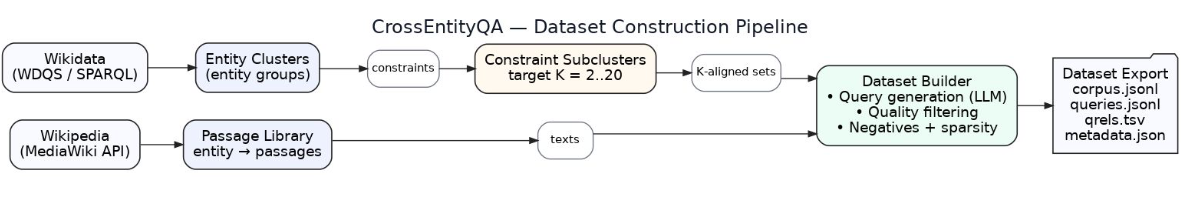
\includegraphics[width=\linewidth]{figures/cross_entity_qa.png}
\caption{CrossEntityQA construction. Wikidata entity groups (WDQS/SPARQL)
are split into constraint subclusters with a target relevance count
$K{=}2$--20; a Wikipedia passage library supplies the texts; the builder
generates LLM queries, filters for quality, and controls negatives and
sparsity, exporting corpus, queries, and qrels.}
\label{fig:ceqa}
\end{figure}

%====================================================================
% === Appendix D: Null-Distribution Diagnostics ===
%====================================================================
\section{Null-Distribution Diagnostics}
\label{app:null}
This appendix verifies that the $p$-values are uniform under the null.
On BEIR FiQA, under the \emph{empirical} null the non-relevant $p$-values
are uniform (KS $p{=}0.13$; 5.0\% below 0.05), whereas a \emph{parametric
normal} null is not (KS $p{=}0.000$, an excess spike near zero), which is
why we keep the empirical null; relevant documents carry systematically
small $p$-values (Cohen's $d{=}{-}1.33$), and the QQ plot of empirical
$p$-values sits on the uniform diagonal (Figure~\ref{fig:nulldiag}).

\begin{figure}[h]
\centering
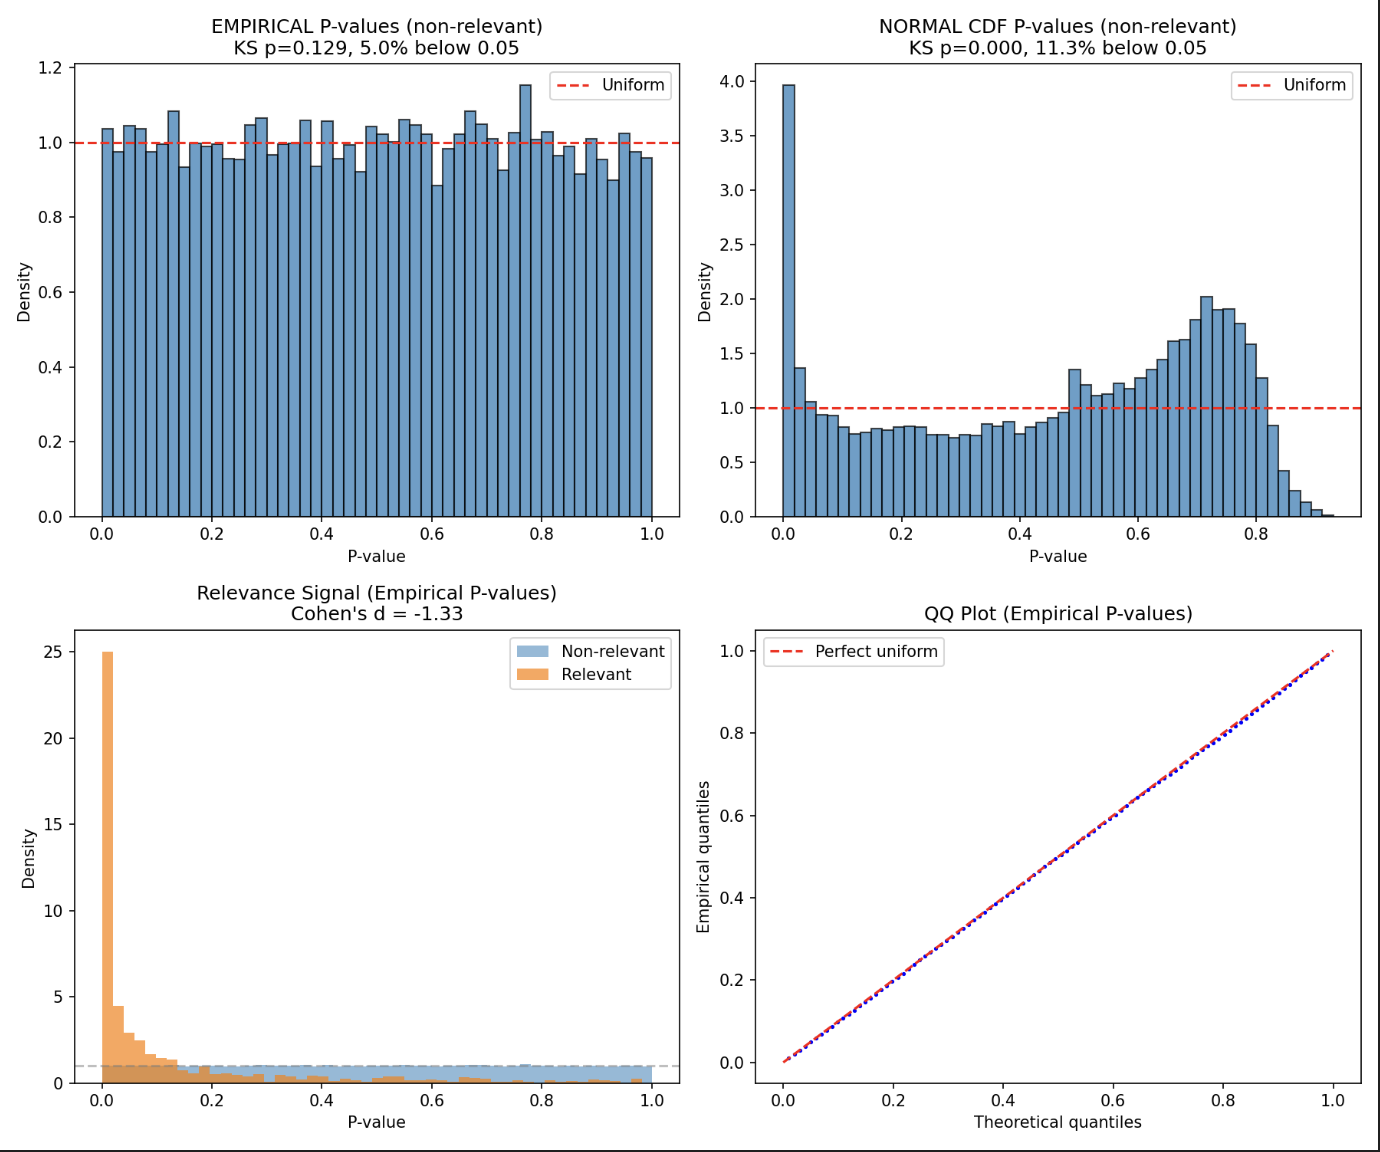
\includegraphics[width=\linewidth]{figures/fiqa_null_pvalues.png}
\caption{$p$-value uniformity diagnostics under the null (BEIR FiQA). The
empirical null is uniform (top-left; QQ bottom-right) while a parametric
normal null is not (top-right); relevant documents separate in $p$-value
space (bottom-left).}
\label{fig:nulldiag}
\end{figure}

%====================================================================
% === References ===
%====================================================================
\bibliography{refs}

\end{document}
